\scanpage{22}
% Folio d'archive : 21 (en haut à gauche) ; pas de pagination autographe distincte.
Il faut aussi considérer des conditions sur un $i:A_0\longrightarrow A$ pour que
\[
\int_{A_0}i^*(\unsure{\xi|\zeta})\xrightarrow{\sim}\int_A\unsure{\xi|\zeta}
\qquad\text{pour tout }\unsure{\xi|\zeta}\in\operatorname{Ob}\mathcal H(A)
\]
(Situation de ``cofinalité''). Si $i$ a un adjoint à
\deleted{\unsure{droite}}\deleted{\unsure{gauche}}\inserted{gauche} $j$
($j,i$ syst. de foncteurs adjoints), je présume que
\figure{\begin{tikzpicture}
\node at (-1.5,0) {?};
\node[draw,ellipse] {$i_{\mathcal H}^*=j_!^{\mathcal H}$};
\node at (1.6,.45) {$*$};
\end{tikzpicture}}
et la formule suit, i.e.
\[
p_{0!}^{\mathcal H}i_{\mathcal H}^*\xrightarrow{\sim}p_!^{\mathcal H}
\quad\text{devient}\quad
p_{0!}^{\mathcal H}\unsure{i_!^{\mathcal H}|j_!^{\mathcal H}}\simeq p_!^{\mathcal H}
\]
qui est \unsure{envisagée|conséquence} car $p_0\unsure{i|j}=p$.
\diagram{\begin{tikzcd}[column sep=large,row sep=large]
A_0\arrow[r,"i"]\arrow[d,"p_0"'] & A\arrow[dl,dash,"p"]\\
\Delta_0 &
\end{tikzcd}}
\margin{Cas des catégories filtrantes ??\quad
(Et foncteurs \unsure{cofinaux} entre ``icelles'')}

\uline{Ex} Cas où $A_0$ réduit à un pt, envoyé dans $e$ objet
final de $A$ : on trouve
\[
\int_A\unsure{\xi|\zeta}\xleftarrow{\sim}\unsure{\xi|\zeta}(e)
\]

$*$ Résulte du diagramme comm. (où on a remplacé $A_0$ par $B$),
valable pour $j:A\longrightarrow B$ quelc. :
\diagram{\begin{tikzcd}[column sep=huge,row sep=large]
\mathcal H(A)\arrow[r,"{(h_A)_!^{\mathcal H}}"]\arrow[d,"{j_!^{\mathcal H}}"'] &
\mathcal H(\widehat A)\arrow[d,"{(j^*_{\wedge})_{\mathcal H}^*}"]\\
\mathcal H(B)\arrow[r,"{(h_B)_!^{\mathcal H}}"'] &\mathcal H(\widehat B)
\end{tikzcd}}
\margin{\uline{NB} dans le cas où $j$ a un adjoint à dr. $i$, on a
$j^*_{\wedge}=i_!^{\wedge}$, qui induit $i:B\longrightarrow A$
donc $(i_!^{\wedge})_{\mathcal H}^*$ induit $i_{\mathcal H}^*$.}
% Petit encadré oblique, sous la marge gauche du dernier diagramme.
\figure{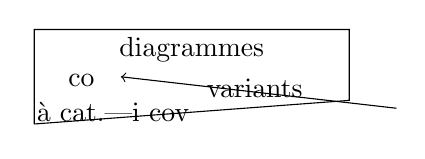
\begin{tikzpicture}
\draw (0,0)--(0,1.2)--(4,1.2)--(4,.3)--(0,0);
\node at (2,.95) {diagrammes};
\node at (.6,.55) {\unsure{co}};
\node at (2.8,.45) {\deleted{\unsure{variants}}};
\draw[->] (4.6,.2)--(1.1,.6);
\node at (1,.15) {\unsure{à cat.|i cov}};
\end{tikzpicture}}
% Inscription pâle renversée à 180 degrés au bord inférieur, barrée.
\deleted{\unsure{Théorie|Flèches}\ \illegible{1}\ \unsure{flèches|fibres}\quad II}
